\documentclass[a4paper]{article}
\usepackage{tikz}
\usepackage{graphicx}
\usepackage{hyperref}
\title{Design Choices and Functionality Definition for ENTIRE EDIH Test before Invest Demonstrator Scheduling}
\author{Liam O'Toole and Helmut Simonis\\School of Computer Science and Information Technology\\University College Cork\\Cork, Ireland\\helmut.simonis@insight-centre.org}
\begin{document}
\maketitle
\begin{abstract}
This document describes the design alternatives and choices made for the demonstrator software used in the "test before invest" service for scheduling in the ENTIRE EDIH. We compare four possible system architectures, and justify our decision or a web-based application with a Java based back-end. We also describe the required functionality, first a minimal viable product definition to test the overall design and obtain some user feedback, then the full functionality intended for the actual service delivery.
\end{abstract}

\section{Introduction}
\label{sec:introduction}

\section{Architecture Design Alternatives}
\label{sec:alternatives}

\begin{itemize}
\item Standalone MiniZinc
\item Jupyter Notebook
\item Desktop application
\item Desktop application with REST
\item Pure REST based solver
\item Web-based aapplication
\end{itemize}


\subsection{Standalone Minizinc Program}

\begin{description}
\item[-] very limited user experience
\item[-] target audience will not be familiar
\item[-] needs installation in customer machines
\item[+] JSON Support in MiniZinc
\item[-] no support for dates/times 
\item[-] Not all scheduling constraints available
\item[-] No support for commercial solvers
\end{description}

\subsection{Jupyter Notebook}

\begin{description}
\item[+] widely used for prototyping
\item[+] very goodd tool support
\item[-] commercial tool support is an issue
\item[-] target audience probably is not familiar
\item[-] unfamiliar with Python interfaces of solvers/ MiniZinc Python interface
\item[-] may require installation on customer machine
\end{description}

\subsection{Desktop Java Application}

\begin{description}
\item[+] based on over ten years of experience developing prototypes
\item[+] full featured JSON interfaces 
\item[+] sophisticated reporting/ presentation features available
\item[-] requires installation in customer machines
\item[-] licence management for commercial tools would be challenging
\item[-] in-app visualization not well supported
\item[-] testing issues when used by end-users
\end{description}

\subsection{Desktop Java Application with REST}

\begin{description}
\item[+] as above, except that commercial tools would be run remotely
\end{description}

\subsection{Pure REST-based Solver}

\begin{description}
\item[+] no installation
\item[-] very limited user experience 
\item[+] close to a deployable application
\item[-] required integration into workflow to be practical
\item[+] existing extension of framework as REST server
\item[-] scalability issue: computing power provided by UCC
\item[-] difficult to debug: not an issue for customers
\end{description}


\subsection{Web-based app}

\begin{description}
\item[+] no installation
\item[+] potential to run on non PC platforms
\item[+] easy to use commercial solvers
\item[-] security concerns/ access control
\item[+] existing extension of framework for backend solver
\item[-] requires development/interface of visualization components
\item[-] scalability issue: computing power provided by UCC
\item[-] difficult to debug: not an issue for customers
\end{description}


\section{Chosen Design}
\label{sec:design}

\begin{enumerate}
\item Back-end solver
\begin{itemize}
\item Define JSON formats
\item Build data model to read/produce JSON files
\item Test harness : Problem generator
\item Write back-end solver based on MiniZinc
\item Write back-end solver based on CPOptimizer  
\end{itemize}
\item Front-end
\begin{itemize}
\item Load/Modify input data from file
\item Call solver
\item Consume results
\item Allow browsing of results
\end{itemize}
\item Integration
\begin{itemize}
\item Test framework on developer machines
\item Production system on UCC/Insight servers
\item Access control mechanism for deployment
\end{itemize}
\end{enumerate}

\begin{figure}[htbp]
\caption{\label{fig:chosendesign}Chosen Design}
\centering
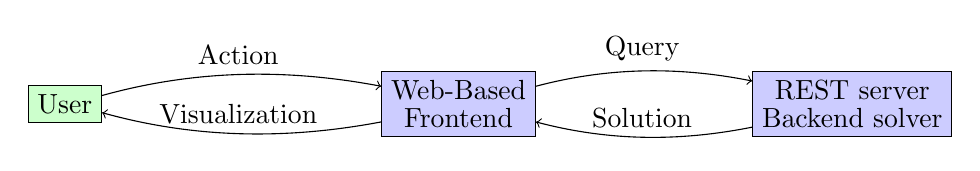
\begin{tikzpicture}[xscale=5,yscale=2]
\node[fill=green!20,draw=black] (user) at (0,1) {User};
\node[fill=blue!20,draw=black] (frontend) at(1,1) {\shortstack{Web-Based\\Frontend}};
\node[fill=blue!20,draw=black] (backend) at (2,1) {\shortstack{REST server\\Backend solver}};
\path[black,bend left,->] (user) edge node[above]{Action}(frontend);
\path[black,bend left,->] (frontend) edge node[above]{Visualization}(user);
\path[black,bend left,->] (frontend) edge node[above]{Query}(backend);
\path[black,bend left,->] (backend) edge node[above]{Solution}(frontend);
\end{tikzpicture}
\end{figure}


\section{MVP: Minimal viable product functionality}
\label{sec:mvp}

\subsection{Constraints}

\begin{itemize}
\item Product, order, job, task
\item end-to-start temporal constraints
\item Release date, soft due date
\item intra-job linear sequence of tasks
\item disjunctive machines
\item cumulative machines
\item machine choice
\item WiP
\item planned shutdown
\end{itemize}

\subsection{Objective}

\begin{itemize}
\item makespan
\item total Lateness
\end{itemize}


\subsection{Visualization}

\begin{itemize}
\item Data lists
\item Job Gantt Chart
\item Machine Gantt Chart
\item Resource Profiles
\end{itemize}

\subsection{Solver Support}

\begin{itemize}
\item MiniZinc (includes CP-SAT)
\item CPOptimizer
\end{itemize}

\section{Planned Full Functionality}
\label{sec:fullfunctionality}

\subsection{Constraints}

\begin{itemize}
\item alternative process paths
\item producer/consumer (component stock, intermediate products
\item calendars
\item skill levels
\end{itemize}


\subsection{Objective}

\begin{itemize}
\item add earliness
\item add flowtime
\item multi-objective
\end{itemize}

\subsection{Visualization}

\begin{itemize}
\item add KPIs
\item add Multi solution
\item add solution comparison
\end{itemize}

\subsection{Solver Support}

\begin{itemize}
\item add CP SAT direct support (if feasible in Java)
\item add OptalCP (if licence can be arranged)
\end{itemize}

\section{Conclusion}
\label{sec:conclusion}

\end{document}
